\documentclass[12pt]{article}

\usepackage{fullpage}
\usepackage{multicol,multirow}
\usepackage{tabularx}
\usepackage{ulem}
\usepackage[utf8]{inputenc}
\usepackage[russian]{babel}
\usepackage{listings}
\usepackage{hyperref}
\usepackage{graphicx}
\usepackage{amsmath}
\usepackage{xcolor}
\DeclareGraphicsExtensions{.png}


\begin{document}

\section*{Лабораторная работа №\,4 по курсу криптографии}

Выполнила студентка группы М8О-307Б \textit{Безлуцкая Елизавета}.

\subsection*{Условие}
Подобрать такую эллиптическую кривую над конечным простым полем порядка p, такую,
порядок точки которой полным перебором находится за 10 минут на ПК. Упомянуть в отчёте
какие алгоритмы и теоремы существуют для облегчения и ускорения решения задачи полного
перебора.

\subsection*{Метод решения}

Я взяла эллиптическую кривую $y^2 = x^3 + ax + b$, выбрала случайным образом коэфициенты $a$ и $b$. С помощью решета Эратосфена сформировала массив простых чисел до 3000 и посмотрела, сколько времени для разных $p$ занимает поиск всех точек кривой и поиск порядка случайно выбранной точки. Получила такой результат:

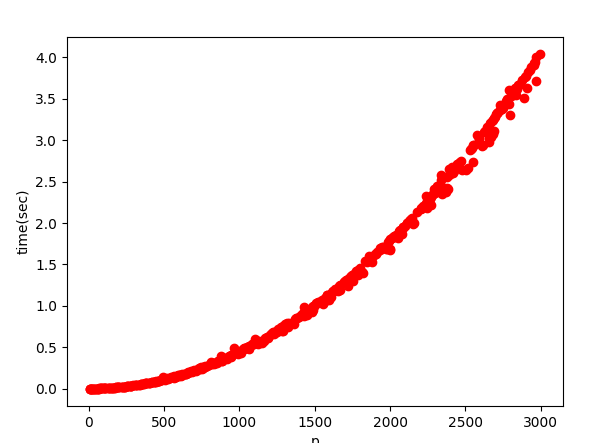
\includegraphics[scale=0.5]{images/ptime.png}

Из данного соотношения прикинула, что $p$ должно быть около 37000.\\

Поиск всех точек занимает много времени, это происходит из-за полного перебора ($\Theta(p^2)$). Далее ищем порядок случайно выбранной из найденных точки. Складываем ее с самой собой до тех пор, пока не получим нулевую точку. Количество операций сложения и будет являться искомым порядком.\\

\subsection*{Исходный код}
\definecolor{codegreen}{rgb}{0,0.6,0}
\definecolor{codegray}{rgb}{0.5,0.5,0.5}
\definecolor{codepurple}{rgb}{0.58,0,0.82}
\definecolor{backcolour}{rgb}{0.95,0.95,0.92}
 
\lstdefinestyle{mystyle}{
    backgroundcolor=\color{backcolour},   
    commentstyle=\color{codegreen},
    keywordstyle=\color{magenta},
    numberstyle=\tiny\color{codegray},
    stringstyle=\color{codepurple},
    basicstyle=\footnotesize,
    breakatwhitespace=false,         
    breaklines=true,                 
    captionpos=b,                    
    keepspaces=true,                 
    numbers=left,                    
    numbersep=5pt,                  
    showspaces=false,                
    showstringspaces=false,
    showtabs=false,                  
    tabsize=2
}
 
\lstset{style=mystyle}
 
\lstinputlisting[language=Python]{code/main.py}

\subsection*{Консоль}
\begin{lstlisting}
y^2 = x^3 + 12987 * x + 32272 (mod 36997)
Elliptic curve group order = 36953
Order of point (17716, 12077): 36953
Time: 624.449035168
\end{lstlisting}

\subsection*{Выводы}
Существует более эффективный алгоритм подсчёта числа точек на эллиптической кривой над конечным полем : алгоритм Шуфа. Он использует теорему Хасее и выполняется за время $O(log^8 q)$.

\end{document}\grid
